\documentclass[a4paper,12pt]{article}
\usepackage{graphicx, amsthm, enumerate, parskip}
\usepackage{amsmath, amssymb, amsthm, amsfonts}
\theoremstyle{definition}
\newtheorem{definition}{Definisi}[section]
\newtheorem{theorem}{Teorema}[section]
\newtheorem{example}{Contoh}[section]
\usepackage{listings, fancyvrb, spverbatim, xcolor}
\lstset{% setup listings
    language=R,% set programming language
    frame=tb,
    basicstyle=\ttfamily\small,% basic font style
    keywordstyle=\color{blue},% keyword style
    commentstyle=\color{gray},% comment style
    breaklines=true,% automatic line breaking
    fancyvrb=true,% verbatim code is typset by listings
}
\usepackage[
    backend=biber,
    style=bwl-FU,
    sorting=nyt,
    maxbibnames=99,
    natbib=true,
]
{biblatex}
\addbibresource{DPustaka.bib}

%% ---------------------------
\begin{document}
    \title{MONTE CARLO INTEFRATION AND VARIANCE REDUCTION}
    \author{Ananda Ravi Shouma Setyawan 4112321004\\
    Novia Rahmadini 4112321024}
\date{\today}
\begin{titlepage}
    \maketitle
\end{titlepage}


\section{Variasi Kontrol}
Pendekatan lain untuk mengurangi varians dalam penaksir Monte Carlo $\theta = E\left [ g\left ( X \right ) \right ]$ digunakan untuk variat kontrol. Misalkan ada fungsi $f$,sehingga $\mu = E\left [ f\left ( X \right ) \right ]$ diketahui, dan $f\left ( X \right )$ berkorelasi dengan $g\left ( X \right )$. Kemudian untuk setiap konstanta $c$, mudah untuk memeriksa bahwa $\widehat{\theta_{c}}=g\left ( X \right )+c\left ( f\left ( X \right )-\mu  \right )$ adalah penaksiran $\theta$ yang tidak bias. 

Variansi
\begin{equation*}
    Var\left ( \widehat{\theta_{c} } \right )=Var\left ( g\left ( X \right ) \right )+c^{2}Var\left ( f\left ( X \right ) \right )+2cCov\left ( g\left ( X \right ) ,f\left ( X \right )\right )
\end{equation*}

adalah fungsi kuadrat dari $c$. ini diminimalkan pada $c=c^{*}$, dimana
\begin{equation}
    c^{*}=-\frac{Cov\left ( g\left ( X \right ),f\left ( X \right ) \right )}{Var\left ( f\left ( X \right ) \right )}
\end{equation}

dan variansi minimum adalah 
\begin{equation}
    Var\left ( \widehat{\theta _{c^{*}}} \right )=Var\left ( g\left ( X \right ) \right )-\frac{\left [ Cov\left ( g\left ( X \right ),f\left ( X \right ) \right ) \right ]^{2}}{Var\left ( f\left ( X \right ) \right )}
\end{equation}

variabel acak $f\left ( X \right )$ disebut variat kontrol untuk penaksirsan $g\left ( X \right )$. di $\left ( 2 \right )$ kita melihat bahwa $Var\left ( g\left (X \right ) \right )$ dikurangi dengan
\begin{equation*}
    \frac{\left [ Cov\left ( g\left ( X \right ),f\left ( X \right ) \right ) \right ]^{2}}{Var\left ( f\left ( X \right ) \right )},
\end{equation*}

maka pengurangan persen dalam varians adalah 
\begin{equation*}
    100\frac{\left [ Cov\left ( g\left ( X \right ),f\left ( X \right ) \right ) \right ]^{2}}{Var\left ( g\left ( X \right ) \right )Var\left ( f\left ( X \right ) \right )}=100\left [ Cor\left ( g\left ( X \right ), f\left ( X \right )\right ) \right ]^{2}
\end{equation*}

dengan demikian, akan menguntungkan jika $f\left (  X\right )$ dan $g\left (X  \right )$ berkorelasi kuat tidak ada pengurangan variansiyang dimungkinkan jika  $f\left (  X\right )$ dan $g\left (X  \right )$ tidak berhubungan. untuk menghitung konstanta $c^{*}$,kita membutuhkan $Cov\left ( g\left ( X \right ),f\left ( X \right ) \right )$ dan $Var\left ( f\left ( X \right ) \right )$, tetapi parameter ini dapat diperkirakan jika perlu, dari Monte awal Eksperimen Carlo.

\begin{example}(Control Variate).
    Menerapkan pendekatan variate kontrol ke komputasi
    \begin{equation*}
        \theta = E\left [ e^{U} \right ]=\int_{0}^{1}e^{u}du,
    \end{equation*}

    dimana $U\sim$ seragam dengan $\left (0,1  \right )$. Dalam contoh ini kita tidak perlu simulasi karena $\theta = e-1=1.718282$ dengan integrasi, tetapi ini memberikan contoh dimana kita dapat memverifikasi bahwa pendekatan variansi kontrol diterapkan dengan benar. Jika pendekatan Monte Carlo sederhanaditerpakan dengan replikasi $m$, variansi dari penaksiran $Var\left ( g\left ( U \right ) \right )/m$, dimana 
    \begin{equation*}
        Var\left ( g\left ( U \right ) \right )=Var\left ( e^{U} \right )=E\left [ e^{2U} \right ]-\theta^{2}=\frac{e^{2}-1}{2}-\left ( e-1 \right )^{2}=0.2420351
    \end{equation*}
    pilihan alami untuk variasi kontrol adalah $U\sim$seragam dengan $\left (0,1  \right )$. kemudian $E\left [ U \right ]=\frac{1}{2},Var=\frac{1}{2}$, dan $Cov\left ( e^{U},U \right )=1-\left ( \frac{1}{2} \right )\left ( e-1 \right )=0.1408591$ maka
    \begin{equation*}
        c^{*}\frac{-Cov\left ( e^{U},U \right )}{Var\left ( U \right )}=-12+6\left ( e-1 \right )=-1.690309
    \end{equation*}
    
    Penaksiran terkontrol kami adalah $\widehat{\theta_{c^{*}}}=e^{U}-1.690309\left (U-0,5  \right )$. untuk m mereplikasi, $mVar\left ( \widehat{\theta_{c^{*}}} \right )$ adalah

    \begin{equation*}
       \begin{split}
            Var\left ( e^{U} \right )-\frac{\left [ Cov\left ( e^{U},U \right ) \right ]^{2}}{Var\left ( U \right )}&=\frac{e^{2}-1}{2}-\left ( e-1 \right )^{2}-12\left ( 1-\frac{e-1}{2} \right )\\
        &=0.2420356-12\left ( 0.1408591 \right )^{2}\\
        &=0.003949175
       \end{split}
    \end{equation*}

    Pengurangan persen varians menggunakan variate kontrol dibandingkan denganperkiraan Monte Carlo sederhana adalah $100(1-0,003940175)/0,2429355 = 98,3781$\% Sekarang kita menerapkan metode variate kontrol untuk masalah ini dan menghitung secara empiris pengurangan persen dalam varians yang dicapai dalam simulasi.Membandingkan perkiraan Monte Carlo sederhana dengan pendekatan variasi kontrol.

    \begin{lstlisting}
        m <- 10000
        a <- - 12 + 6 * (exp(1) - 1)
        U <- runif(m)
        T1 <- exp(U) #simple MC
        T2 <- exp(U) + a * (U - 1/2) #controlled
    \end{lstlisting}   
    memberikan hasil sebagai berikut\\
    \begin{lstlisting}
        > mean(T1)
        [1] 1.717834
        > mean(T2)
        [1] 1.718229
        > (var(T1) - var(T2)) / var(T1)
        [1] 0.9838606
    \end{lstlisting}
\end{example}

menggambarkan bahwa persentase pengurangan 98,3781\% dalam varians yang diturunkan di atas adalah
kira-kira dicapai dalam simulasi ini.

\begin{example}(Integrasi MC menggunakan variasi kontrol). Gunakan metode dari kontrol bervariasi untuk memperkirakan
\begin{equation*}
    \int_{0}^{1} \frac{e^{-x}}{1 + x{2}}
\end{equation*}
Versi dari masalah ini muncul di ${69,p. 734}$  Parameter yang menarik adalah $ 0= E[g(x)]$ dan g(x) =e $- x/\left ( 1+ x 2 \right )$ dimana X terdistribusi secara merata
pada $(0,1)$ Kami mencari fungsi "dekat" ke g (x) dengan nilai yang diharapkan diketahui, misalnya
bahwa g (x) dan f (x) berkorelasi kuat. Misalnya, fungsi f(x) = e $-5\left ( 1+ x2 \right ) -1$ adalah "dekat" dengan g(x) pada $(0,1)$ dan kita dapat menghitung ekspektasinya. Jika U terdistribusi secara merata pada $(0,1)$ maka
\begin{equation*}
    E[F\left ( U  \right )]e^{-.5}\int_{0}^{1}\frac{1}{1+u^{2}}du=e^{-.5}arctan\left ( 1 \right )=e^{-.5}\frac{\pi }{4}
\end{equation*} 
Menyiapkan simulasi awal untuk mendapatkan estimasi konstanta, kami juga mendapatkan perkiraan$Cor ( g (U) F (U)\cong 0.974$
\begin{lstlisting}
    f < - function ( u )
    exp (-. 5) / ( 1+ u^ 2)
    g < - function (u)
    exp (-u) / ( 1+ u^2)

    set.seed(510) #needed later
    u <- runif (10000)
    b <- f (u)
    A <- g(u) 
\end{lstlisting}
Estimasi dari $c^{*}$ dan $Cor\left ( f\left ( U \right ),g\left ( U \right ) \right )$ adalah\\

\begin{lstlisting}
    > cor(A, B)
    [1] 0.9740585
    a <- -cov(A,B) / var(B) #est of c*
    > a
    [1] -2.436228
\end{lstlisting}
Hasil simulasi dengan dan tanpa kontrol bervariasi mengikuti\\

\begin{lstlisting}
    m <- 100000
    u <- runif(m)
    T1 <- g(u)
    T2 <- T1 + a * (f(u) - exp(-.5)*pi/4)
    > c(mean(T1), mean(T2))
    [1] 0.5253543 0.5250021
    > c(var(T1), var(T2))
    [1] 0.060231423 0.003124814
    > (var(T1) - var(T2)) / var(T1)
    [1] 0.9481199
\end{lstlisting}   

Di sini perkiraan pengurangan varian $g(X)$ dibandingkan dengan $g(X)+\widehat{c^{*}}\left ( f\left ( X \right )-\mu  \right )$adalah 95 persen. Kami akan kembali ke masalah ini untuk menerapkan pendekatan lain untuk pengurangan varians, metode sampling penting.
\end{example} 

\subsection{variate antitetik sebagai variate kontrol}
Penaksir variat antitesis pada bagian sebelumnya sebenarnya merupakan kasus khusus dari penaksir variat kontrol.khusus dari penaksir ragam kontrol. Pertama, perhatikan bahwa penaksir variat kontrol adalah kombinasi linear dari penaksir tak bias dari $\theta$. Secara umum, jika $\widehat{\theta _{1}}$ dan $\widehat{\theta _{2}}$ adalah dua penaksir tak bias dari $\theta$, maka untuk setiap konstanta $c$,
\begin{equation*}
    \widehat{\theta_{c}}=c\widehat{\theta_{1}}+\left ( 1-c \right )\widehat{\theta_{2}}
\end{equation*}
juga tidak bias untuk $\theta$. Variansi dari $c\widehat{\theta_{1}}+\left ( 1-c \right )\widehat{\theta_{2}}$ adalah
\begin{equation}
    Var\left ( \widehat{\theta_{2}} \right )+c^{2}Var\left ( \widehat{\theta_{1}}-\widehat{\theta_{2}} \right )+2cCov\left ( \widehat{\theta_{2}}\widehat{\theta_{1}}-\widehat{\theta_{2}} \right )
\end{equation}
Dalam kasus khusus dari variasi antitesis pada (6.7) dan (6.8), $\widehat{\theta_{1}}$ dan $\widehat{\theta_{2}}$ adalah
berdistribusi identik dan $Cor\left ( \widehat{\theta_{1}},\widehat{\theta_{2}} \right )=-1$. Maka $Cov\left ( \widehat{\theta_{1}},\widehat{\theta_{2}} \right )=-Var\left ( \widehat{\theta_{1}} \right )$, dan varians dalam (3) adalah
\begin{equation*}
    Var\widehat{\theta_{c}}=4c^{2}Var\left ( \widehat{\theta_{1}} \right )+Var\left ( \widehat{\theta_{1}} \right )=\left ( 4c^{2}-4c+1 \right )Var\left ( \widehat{\theta_{1}} \right )
\end{equation*}
dan konstanta optimalnya adalah $c*=\frac{1}{2}$. Penaksir variabel kontrol dalam kasus ini adalah
\begin{equation*}
\widehat{\theta_{c*}}=\frac{\widehat{\theta_{1}}+\widehat{\theta_{2}}}{2}
\end{equation*}
yang (untuk pilihan $\widehat{\theta_{1}}$ dan $\widehat{\theta_{2}}$) merupakan penaksir variabel antitesis dari $\theta$
\subsection{Beberapa variasi kontrol}
Penggabungan penaksir tak bias dari parameter target $\theta$ untuk
mengurangi varians dapat diperluas ke beberapa variabel kontrol. Secara umum, jika $E\left [ \widehat{\theta_{i}} \right ]=\theta,i=1,2,...k$ dan $c=\left ( c_{1},...,c_{k} \right )$ seperti yang $\sum_{i=1}^{k}c_{i}=1$ lalu
\begin{equation*}
    \sum_{i=1}^{k}c_{1}\widehat{\theta_{i}}
\end{equation*}
juga tidak bias untuk $\theta$. Penaksir variabel kontrol yang sesuai adalah
\begin{equation*}
    \widehat{\theta_{c}}=g\left ( X \right )+\sum_{i=1}^{k}c^{*}_{i}\left ( f_{i}\left ( X \right ) -\mu _{i}\right )
\end{equation*}
dimana $\mu _{i}=E\left [ f_{i}\left ( X \right ) \right ],i=,...,k$, dan 
\begin{equation*}
    E\left [ \widehat{\theta_{c}} \right ]=E\left [ g\left ( X \right ) \right ]+\sum_{i=1}^{k}c^{*}_{i}E\left [ f_{i}\left ( X \right )-\mu _{i} \right ]=\theta
\end{equation*}
penaksiran terkontrol $\widehat{\theta_{\widehat{c*}}}$ , dan penaksiran untuk konstanta optimal $c^{*}_{i}$, dapat diperoleh dengan melakukan fitting model regresi linier.

\subsection{variabel kontrol dan regresi}
Pada bagian ini kita akan membahas kaitan antara pendekatan variabel kontrol dan regresi linier sederhana. Hal ini memberikan lebih banyak wawasan tentang bagaimana variasi kontrol mengurangi varian dalam integrasi Monte Carlo. Selain itu, kami memiliki metode yang mudah digunakan untuk mengestimasi konstanta optimal $c^{*}$, parameter target, persen pengurangan varians, dan kesalahan standar estimator, semuanya dengan menyesuaikan model regresi linier sederhana.

Misalkan $\left ( X_{1},Y_{1} \right ),...,( X_{n},Y_{n} )$ ) adalah sampel acak dari distribusi bivariat dengan berarti $\left ( \mu _{X},\mu _{Y} \right )$ dan varians $\left ( \sigma ^{2}_{X},\sigma ^{2}_{y} \right )$. Mari kita bandingkan penaksir kuadrat terkecil untuk regresi $X$ terhadap $Y$ dengan penaksir estimator variabel kontrol.
Jika terdapat hubungan linier $X=\beta _{1}Y+\beta _{0}+\epsilon $, dan $E\left [ \epsilon  \right ]=0$, maka
\begin{equation*}
    E\left [ E \right ]=E\left [ E\left [ E\left [ Y \right ] \right ] \right ]=E\left [ \beta _{0}+\beta_{1}Y+\epsilon  \right ]=\beta_{0}+\beta_{1\mu Y}
\end{equation*}
disini $\beta{0}$ dan $\beta_{1}$ adalah parameter konstan dan $\epsilon$ adalah variabel acak. mari kita pertimbangkan sampel bivariat $\left ( g\left ( X_{1} \right ),f\left ( X_{1} \right ) \right ),...,\left ( g\left ( X_{n} \right ),f\left ( X_{n} \right ) \right )$. Sekarang jika $g(X)$ menggantikan $X$
dan $f(X)$ menggantikan $Y$, kita memiliki $g\left ( X \right )=\beta_{0}+\beta_{1}f(X)+\epsilon$, dan 
\begin{equation*}
    E\left [ g\left ( X \right ) \right ]=\beta_{0}+\beta_{1}\left [ f(X) \right ]
\end{equation*}
Estimator kuadrat terkecil dari kemiringan adalah
\begin{equation*}
    \widehat{\beta_{1}}=\frac{\sum_{i=1}^{n}(X_{i}-\overline{X})(Y_{i}-\overline{Y})}{\sum_{i=1}^{n}(Y_{i}-\overline{Y})}=\frac{\widehat{Cov}(X,Y)}{\widehat{Var}(Y))}=\frac{\widehat{Cov}(g(X),f(X))}{\widehat{Var}(f(X))}=-\widehat{c^{*}}
\end{equation*}
Hal ini menunjukkan bahwa cara yang mudah untuk mengestimasi $c^{*}$ adalah dengan menggunakan estimasi kemiringan dari model regresi linier sederhana $g(X)$ terhadap $f(X)$:
\begin{lstlisting}
    L <- lm(gx ~ fx)
    c.star <- -L$coeff[2]
\end{lstlisting}
Estimator kuadrat terkecil dari intersep adalah $\widehat{\beta_{0}}=\overline{g(X)}-(-\widehat{c^{*}}\overline{f(X)}$. Sehingga respon yang diprediksi pada $\mu = E\left [ f\left ( X \right ) \right ]$ adalah 
\begin{equation*}
    \begin{split}
        \widehat{\beta_{0}}+\widehat{\beta_{1\mu}}&=\overline{g(x)}+\widehat{c^{*}}(\overline{f(X)}-\widehat{c^{*}}\mu)\\
        &=\overline{g(x)}+\widehat{c^{*}}(\overline{f(X)}-\mu)=\widehat{\theta_{\widehat{c^{*}}}}
    \end{split}
\end{equation*}
kesalahan mean squared error (MSE). Estimasi varians dari penaksir varians kontrol adalah
\begin{equation*}
    \begin{split}
        \widehat{Var}(\overline{g(X)}+\widehat{c^{*}}(\overline{f(X)}-\mu)&=\frac{\widehat{Var}(g(X)+\widehat{c^{*}}(f(X)-\mu))}{n}\\
        &=\frac{\widehat{Var}(g(X)+\widehat{c^{*}}(f(X))}{n}\\
        &=\frac{\widehat{\sigma ^{2}_{\varepsilon }}}{n}
    \end{split}
\end{equation*}

Dengan demikian, estimasi kesalahan standar dari estimasi variabel kontrol dapat dengan mudah dihitung menggunakan $R$ dengan menerapkan metode ringkasan pada objek lm dari dari model regresi yang telah disesuaikan, misalnya dengan menggunakan

\begin{lstlisting}
    se.hat <- summary(L)$sigma
\end{lstlisting}
Untuk mengekstraksi nilai dari $\widehat{\sigma _{\varepsilon }}\sqrt{MSE}$
terakhir, ingatlah bahwa proporsi pengurangan varians untuk kontrol variat adalah $\left [ Cor(g(X),f(X)) \right ]^{2}$Dalam model regresi linier sederhana, nilai koefisien determinasi adalah angka yang sama $(R^{2})$, yang merupakan proporsi total variasi dalam $g(X)$ tentang rata-rata yang dijelaskan oleh $f (X)$.
\begin{example}
(kontrol variasi dan regresi). Kembali ke Contoh 6.8,
mari kita ulangi estimasi dengan memasang model regresi. Dalam masalah ini,
\begin{equation*}
    f(x)=e^{-.5}(1+x^{2})^{-1},0< x< 1
\end{equation*}
dengan $\mu=E\left [f(X)  \right ]=e^{1.5}\pi /4$Untuk mengestimasi konstanta $c{*}$, sesuaikan model linier
meregresikan $g(x)$ pada variabel kontrol $f (x)$. Ekstrak koefisien kemiringan dan tetapan $\widehat{c^{*}}=-\widehat{\beta_{1}}$
\begin{lstlisting}
    set.seed(510)
    mu <- exp(-.5)*pi/4
    u <- runif(10000)
    f <- exp(-.5)/(1+u^2)
    g <- exp(-u)/(1+u^2)
    L <- lm(g ~ f)
    L
    c.star <- - L$coeff[2]
    > c.star
    f
-2.436228
\end{lstlisting}
Kami menggunakan bilangan acak yang sama seperti pada Contoh 6.8 dan mendapatkan taksiran yang sama untuk $c^{*}$. Sekarang $\widehat{\theta_{c^{*}}}$ adalah respon yang diprediksi pada titik $\mu = 0.4763681$, jadi
\begin{lstlisting}
    theta.hat <- sum(L$coeff * c(1, mu)) #pred. value at mu
\end{lstlisting}
Estimasi $\widehat{\theta}$, kesalahan kuadrat rata-rata residual dan proporsi pengurangan dalam varians (R-kuadrat) sesuai dengan taksiran yang diperoleh dalam Contoh 6.8.
\begin{lstlisting}
    > theta.hat
    [1] 0.5253113
    > summary(L)$sigma^2
    [1] 0.003117644
    > summary(L)$r.squared
    [1] 0.9484514
\end{lstlisting}
Jika beberapa variabel kontrol digunakan, maka seseorang dapat mengestimasi model linier
\begin{equation*}
    X=\beta _{0}+\sum_{i=1}^{k}\beta_{1}Y_{i}+\varepsilon 
\end{equation*}
untuk mengestimasi konstanta optimal $c^{*}=(c^{*}_{1},...,c^{*}_{k}$. Kemudian $-\widehat{c^{*}}=(\widehat{\beta_{1}},...,\beta_{k})$dan estimasi tersebut merupakan perkiraan $\widehat{X}$ pada titik $\mu=(\mu_{1},...,\mu_{k}$ Estimasi varians dari penaksir terkendali sekali lagi adalah $\widehat{\sigma^{2}}_{\varepsilon }=MSE/n$ i mana $n$ adalah ukuran sampel (jumlah ulangan, dalam hal ini dalam kasus ini).
\end{example}
\begin{example}
    Contoh 6.10 (Variasi kontrol dan regresi, lanjutan). Melanjutkan Contoh 6.9, mari kita tambahkan variabel kontrol kedua dan gunakan regresi berganda untuk mengestimasi $c^{*}$, yang untuk dua variabel kontrol adalah vektor $c^{*}=(c^{*}_{1},c^{*}_{2}$. disini 
    \begin{equation*}
        g(x)=\frac{e^{-x}}{1+x^{2}},0=\int_{0}^{1}g(x)dx,
    \end{equation*}
    dan variabel kontrolnya adalah
    \begin{equation*}
        f_{1}(u)=\frac{e^{-.5}}{(1+u^{2})}, f_{2}=\frac{e^{-u}}{1-e^{-1}},0<u<1,
    \end{equation*}
    dengan
    $\mu=(\mu_{1},\mu_{2})=(E\left [ f_{1}(U) \right ],E\left [ f_{2}(U) \right ])=(e^{-0.5}\pi/4,1)=(0.476381,1)$
    \begin{lstlisting}
        u <- runif(10000)
    f1 <- exp(-.5) / (1 + u^2)
    f2 <- exp(-u) / (1 - exp(-1))
    g <- exp(-u) / (1 + u^2)
    ## fit the multiple regression with two predictors
    L2 <- lm(g ~ f1 + f2)
> L2$coeff
(Intercept) f1 f2
-0.3345326 0.0240755 1.3414141
> c.star <- - L2$coeff[2:3]
> c.star
f1 f2
-0.0240755 -1.3414141
> mu
[1] 0.4763681 1.7182818
    \end{lstlisting}
    Kami menemukan bahwa estimasi optimal $c^{*}$ adalah
    \begin{equation*}
        \widehat{c^{*}}=(\widehat{c^{*}_{1}},\widehat{c^{*}_{2}})=(-0.0240755,-1.3414141).
    \end{equation*}
    Maka $\widehat{\theta}$ adalah respons yang diprediksi pada $\mu$ dan estimasi varians dari kontrol estimator adalah $MSE/m$, di mana $m$ adalah jumlah ulangan dalam simulasi
    \begin{lstlisting}
        theta.hat <- sum(L2$coeff * c(1, mu)) #pred. value at mu
    theta.hat
    ## alternately
    df <- data.frame(f1=mu1, f2=mu2)
    theta.hat <-predict(L2, df)
    ## MSE / n is the est. variance of the control estimator
    MSE <- summary(L2)$sigma^2
    MSE
    sqrt(MSE / 10000)
    > c.star
        f1             f2
    -0.0240755 -0.8479354
    > theta.hat
             1
    0.5248716
    > MSE
    [1] 5.889139e-05
    \end{lstlisting}
\end{example}
estimasinya adalah $\widehat{\theta}=0.5248716$ dan $MSE=5.89e-05$ dan estimasinya dari $\widehat{\theta_{c^{*}}}$. Bandingkan hal ini dengan estimasi sebelumnya dengan menggunakan MC naif $(\widehat{\sigma_{MC}})=0.060231423$ dan satu variat kontrol$(\widehat{\sigma^{2}_{C}}=0,003117644)$.Hitunglah persen pengurangan varians untuk masing-masing. Ini adalah rata-rata tertimbang dari nilai $R^{2}$, tetapi akan lebih mudah untuk menghitung persen pengurangan varians secara langsung. Dalam rasio Dalam rasio, penyebut 10000 dalam $MSE(\widehat{\theta})$ dibatalkan dari setiap suku.
\begin{lstlisting}
    var0 <- 0.060231423 #naive MC
    var1 <- 0.003117644 #one control variate
    var2 <- summary(L)$sigma^2 #new estimator
    # percent reduction in variance
    100 * (var0 - var1) / var0
    100 * (var1 - var2) / var1
    100 * (var0 - var2) / var0
    > 100 * (var0 - var1) / var0
    [1] 94.82389
    > 100 * (var1 - var2) / var1
    [1] 98.11103
    > 100 * (var0 - var2) / var0
    [1] 99.90222
\end{lstlisting}
Persentase pengurangan ini masing-masing adalah $94,82, 98,90, dan 99,90$
Menurut WolframAlpha,$\theta\cong 0.524797$.Dengan integrasi numerik dalam $R$,$\theta=0,5247971$ dengan kesalah absolut $<5,8e-15$. Estimasi kami untuk $\theta$ adalah $0,5253113$ dan $0,5248716$ dengan satu dan dua metode variasi kontrol, masing-masing.
\section{Sampling Penting}
Nilai rata-rata fungsi g(x) pada interval (a,b) biasanya ditentukan (dalam kalkulus) oleh
\begin{equation*}
    \frac{1}{b-a}\int_{a}^{b}g(x)dx
\end{equation*}
Di sini fungsi bobot seragam diterapkan pada seluruh interval $(a,b)$. Jika X adalah variabel acak terdistribusi secara merata pada $(a,b)$, maka
\begin{equation}
    E\left [ g(X) \right ]=\int_{a}^{b}g(x)\frac{1}{b-a}dx=\frac{1}{b-a}\int_{b}^{a}g(x)dx
\end{equation}
yang merupakan nilai rata-rata dari fungsi $g(x)$ selama interval $(a, b)$ sehubungan dengan fungsi bobot yang seragam. Metode Monte Carlo sederhana menghasilkan sejumlah besar ulangan$X_{1},...,X_{m}$ terdistribusi secara merata $[a, b]$ dan taksiran $\int_{a}^{b}g(x)dx$ dengan rata rata sampel
\begin{equation*}
    \frac{b-a}{m}\sum_{i=1}^{m}g(X_{i})
\end{equation*}
yang konvergen ke $\int_{a}^{b}g(x)dx$ dengan probabilitas 1 dengan hukum kuat besar angka. Salah satu batasan dari metode ini adalah tidak berlaku untuk interval tak bebas. Kelemahan lainnya adalah tidak efisien untuk mengambil sampel secara uniformal melintasi interval jika fungsi $g(x)$ tidak terlalu seragam.
Namun, begitu kita melihat masalah integrasi sebagai masalah nilai yang diharapkan (6.12), tampaknya masuk akal untuk mempertimbangkan fungsi bobot lain (kepadatan lain) selain fungsi seragam. Ini membawa kita ke metode umum yang disebut sampling penting

Misalkan $X$ adalah variabel acak dengan fungsi kerapatan $f(x)$, sehingga $f(x) > 0$ pada himpunan ${x : g(x) > 0}$. Biarkan $Y$ menjadi variabel acak $g(X)/f(X)$.Kemudian
\begin{equation*}
    \int g(x)dx=\int \frac{g(x)}{f(x)}f(x)dx=E\left [ Y \right ]
\end{equation*}
Perkirakan $E[Y]$ dengan integrasi Monte Carlo sederhana. Artinya, menghitung rata-rata
\begin{equation*}
    \frac{1}{m}\sum_{i=1}^{m}Y_{i}=\frac{1}{m}\sum_{i=1}^{m}\frac{g(X_{i})}{f(X_{i})}
\end{equation*}
where the random variables$ X_{1}, . . . , X_{m}$ are generated from the distribution with density $f(x)$. The density $f(x)$ is called the importance function.
Dalam metode pengambilan sampel kepentingan, varian dari estimator didasarkan
pada $Y = g(X)/f(X)$ adalah $Var(Y)/m$, sehingga variansi$Y$ harus kecil. Itu variansi $Y$ kecil jika $Y$ hampir konstan, sehingga kerapatan $f(.)$ seharusnya mendekati ke $g(x)$. Juga, variabel dengan kerapatan $f(.)$ seharusnya cukup mudah untuk mensimulasikan.
\begin{example}
    Dalam Contoh 6.5, random normal dihasilkan untuk menghitung Monte Estimasi Carlo dari cdf normal standar, $\phi (2)=P(X\leq 2)$.Dalam naif Pendekatan Monte Carlo, pendugaan pada ekor distribusi kurang tepat.Secara intuitif, kita mungkin mengharapkan perkiraan yang lebih tepat untuk ukuran sampel tertentu jika distribusi yang disimulasikan tidak seragam. Dalam hal ini, rata-rata harus menjadi rata-rata tertimbang darpada rata-rata sampel yang tidak tertimbang, untuk mengoreksi untuk bias ini. Metode ini disebut sampling kepentingan (lihat Robert and Casella [240, Sec. 3.3]). Keuntungan dari sampling kepentingan adalah bahwa distribusi sampling kepentingan dapat dipilih sehingga varians dari Monte Estimator Carlo berkurang.
    Misalkan $f(x)$adalah kerapatan yang didukung pada himpunan $A$. Jika $\phi(x)>0$ pada $A$.kemudian integral
    \begin{equation*}
        \theta=\int_{A}g(x)f(x)dx,
    \end{equation*}
    dapat dituliskan
    \begin{equation*}
        \theta=\int_{A}g(x)\frac{f(x)}{\phi (x)}\phi(x)dx
    \end{equation*}
    jika $\phi(x)$ adalah kerapatan di A, maka estimator dari $\theta=E_{\phi}\left [ g(x)f(x)/\phi (x) \right ]$ adalah
    \begin{equation*}
        \widehat{\theta}\frac{1}{n}\sum_{i=1}^{n}g(X_{i})\frac{f(X_{i})}{\phi(X_{i})}
    \end{equation*}
    dimana $X_{1},...,X_{n}$ adalah sampel acak dari kepadatan $\phi(x)$. fungsi disebut $\phi(.)$ disebut amplop atau fungsi pengambilan sampel penting. ada banyak kepadatan $\phi(x)$ yang nyaman untuk disimulasikan
    biasanya seseorang harus memilih $\phi(x)$ sehingga $\phi (x)\cong \left | g(x) \right |f(x)$ pada $A$ (dan $\phi(x) memiliki varian yang terbatas$)
\end{example}
\begin{example}
        (Pilihan fungsi kepentingan). Dalam contoh ini (dari[69, hal. 728]) beberapa kemungkinan pilihan fungsi kepentingan untuk diestimasi
        \begin{equation*}
            \int_{0}^{1}\frac{e^{-x}}{1+x^{2}}dx
        \end{equation*}
        dengan metode sampling kepentingan dibandingkan. Kandidat untuk fungsi kepentingan adalah
        \begin{equation*}
            \begin{split}
                f_{0}(x)&=1, 0<x<1,\\
                f_{1}(x)&=e^{-x},0<x<\infty\\
                f_{2}(x)&=(1+x^{2})^{1}/\pi,-\infty<x<\infty\\
                f_{3}(x)&=e^{-x}/(1-e^{-1}),o<x<1\\
                f_{4}(x)&=4(1+x^{2})^{-1}/\pi,0<x<1
            \end{split}
        \end{equation*}
        Integrannya adalah
        \begin{equation*}
            g(x)=\left\{\begin{matrix}
            e^{-x}/(1+x^{2}),  &  &jika (0<x<1) \\ 
            0 &  & jika \ tidak
            \end{matrix}\right.
        \end{equation*}
        Sementara kelima fungsi kepentingan yang mungkin adalah positif di set $0 < x < 1$ di mana$ g(x) > 0$, $f_{1}$ dan $f_{2}$ memiliki rentang yang lebih besar dan banyak nilai yang disimulasikan akan memberi kontribusi nol pada penjumlahan, yang tidak efisien. Semua distribusi ini mudah disimulasikan; $f_{2}$ adalah standar Cauchy atau $t(v=1)$.
        Kepadatan diplot pada $(0,1)$ untuk dibandingkan dengan $g(x)$ pada Gambar 6.1(a). Fungsi yang sesuai dengan rasio paling mendekati konstan $g(x)/f(x)$ tampaknya $f_{3}$, yang dapat dilihat lebih jelas pada Gambar 6.1(b). Dari grafik, kita mungkin lebih suka $f_{3}$ untuk varians terkecil.
\begin{lstlisting}
m <- 10000
theta.hat <- se <- numeric(5)
g <- function(x) {
exp(-x - log(1+x^2)) * (x > 0) * (x < 1)
}
x <- runif(m) #using f0
fg <- g(x)
theta.hat[1] <- mean(fg)
se[1] <- sd(fg)
x <- rexp(m, 1) #using f1
fg <- g(x) / exp(-x)
theta.hat[2] <- mean(fg)
se[2] <- sd(fg)
x <- rcauchy(m) #using f2
i <- c(which(x > 1), which(x < 0))
x[i] <- 2 #to catch overflow errors in g(x)
fg <- g(x) / dcauchy(x)
theta.hat[3] <- mean(fg)
se[3] <- sd(fg)
u <- runif(m) #f3, inverse transform method
x <- - log(1 - u * (1 - exp(-1)))
fg <- g(x) / (exp(-x) / (1 - exp(-1)))
theta.hat[4] <- mean(fg)
se[4] <- sd(fg)
u <- runif(m) #f4, inverse transform method
x <- tan(pi * u / 4)
fg <- g(x) / (4 / ((1 + x^2) * pi))
theta.hat[5] <- mean(fg)
se[5] <- sd(fg)
\end{lstlisting}
        Kode untuk menampilkan Gambar 6.1(a) dan 6.1(b) diberikan di akhir bab ini.
        
        \begin{figure}[h]
        \centering
        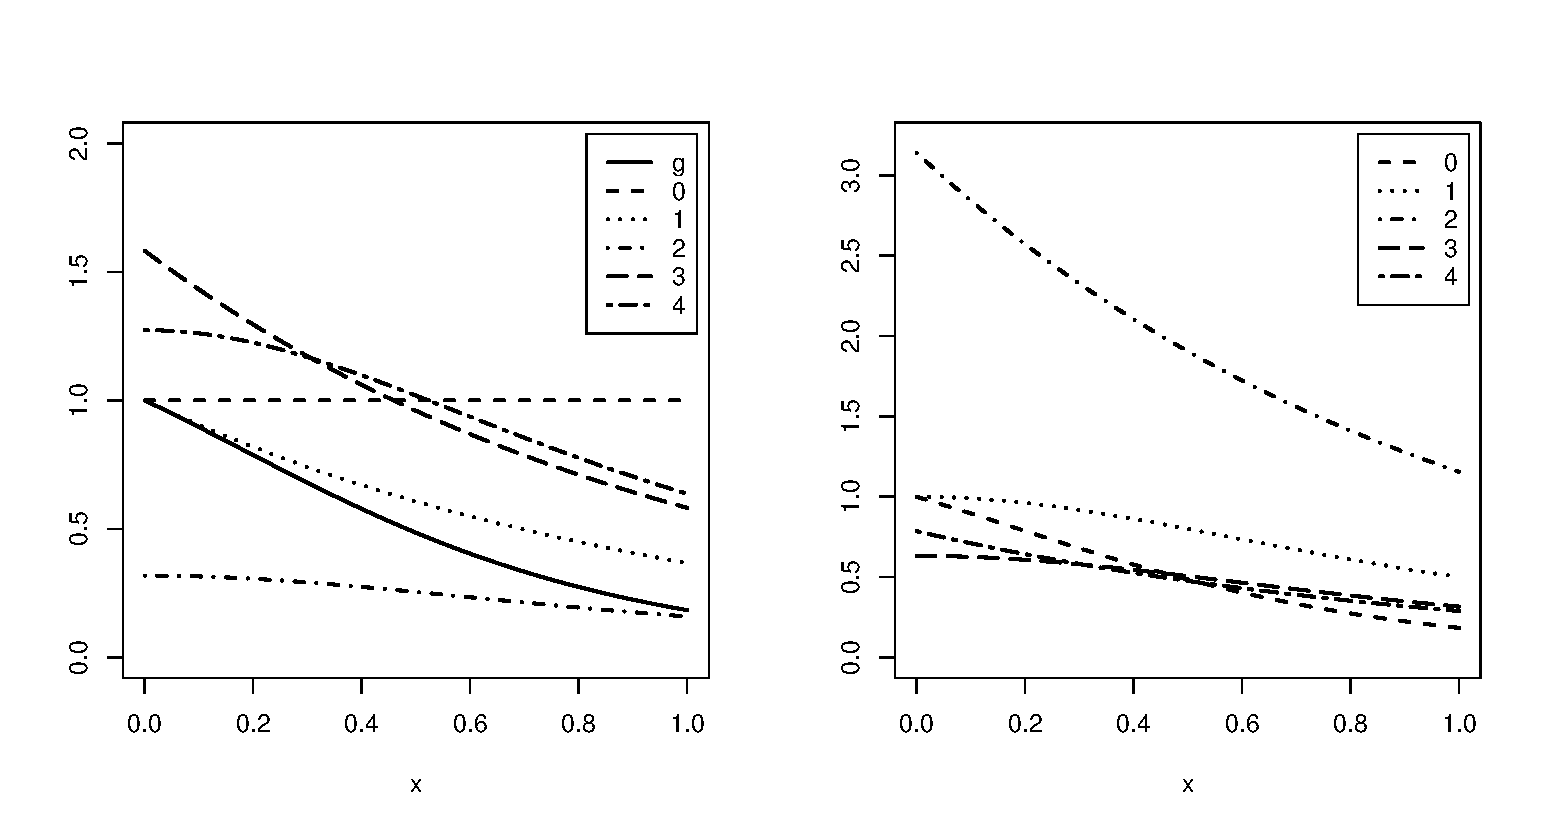
\includegraphics [width=\textwidth]{gb/K5G1}
        \caption{: Pentingnya fungsi pada Contoh 2.2: $f_{0}$, . . . ,$ f_{4}$ (baris 0:4)dengan $g(x)$ dalam $(a)$ dan rasio $g(x)/f(x)$ dalam (b).}
        \label{fig:my_label}
        \end{figure}
        Estimasi (diberi label theta.hat) dari$\int_{0}^{1}g(x)dx$ dan yang sesuai kesalahan standar se untuk simulasi menggunakan masing-masing fungsi penting adalah
        \begin{lstlisting}
        > rbind(theta.hat, se/sqrt(m))
        [,1]        [,2]      [,3]         [,4]     [,5]
         theta.hat 0.524114007 0.531358351 0.5461507 0.5250698759 0.526049238
        0.002436559 0.004181264 0.0096613 0.0009658794 0.001427685
        \end{lstlisting}
        jadi simulasi menunjukkan bahwa $f_{3}$ dan kemungkinan $f_{4}$ menghasilkan varian terkecil di antara kelima fungsi kepentingan tersebut, sedangkan $f_{2}$ menghasilkan varian tertinggi.Estimasi standar Monte Carlo tanpa pengambilan sampel penting memiliki $\widehat{se}=0,244(f_{0}=1)$. Fungsi kepentingan $f_{1}$ dan $f_{2}$ tidak mengurangi kesalahan, tetapi $f_{3}$ dan $f_{4}$ masing-masing mengurangi kesalahan standar dalam memperkirakan $\theta$.
        
        Densitas Cauchy $f_{2}$ didukung pada seluruh garis real, sedangkan in tegrand $g(x)$ dievaluasi pada (0,1). Ada sejumlah besar angka nol(sekitar 75\%) dihasilkan dalam rasio $g(x)/f(x)$ dalam kasus ini, dan semua nilai lainnya jauh dari 0, menghasilkan varian yang besar. Berikut ringkasan statistik untuk rasio $g(x)/f_{2}(x)$ mengkonfirmasi hal ini.
        \begin{lstlisting}
            Min. 1st Qu. Median Mean 3rd Qu. Max.
         0.0000 0.0000 0.6891 0.5314 0.9267 1.0000
        \end{lstlisting} 
        Contoh 2.2 mengilustrasikan bahwa kehati-hatian harus diambil untuk memilih kepentingan fungsi yang menghasilkan varian kecil $Y = g(X)/f(X)$. Pentingnya fungsi harus berupa $f$ yang didukung tepat pada himpunan di mana $g(x) > 0$, dan sehingga rasio $g(x)/f(x)$ hampir konstan.
    \end{example}
    \subsection{Variansi dalam Pengambilan Sampel Kepentingan}
    jika $\phi(x)$ adalah distribusi sampling kepentingan. $f(x)=1 pada A$ dan $X$ FKP $\phi(x)$ didukung pada A, kemudian
    \begin{equation*}
        \theta=\int_{A}g(x)dx= \int_{A}\frac{g(x)}{\phi(x)}\phi (x)dx=E\left [ \frac{g(X)}{\phi(X)} \right ]
    \end{equation*}
    jika $X_{1},...,X_{n}$ adalah sampel acak dari distribusi X, estimator lagi sampel-rata-rata
    \begin{equation*}
        \widehat{\theta}=\overline{g(X)}=\frac{1}{n}\sum_{i=1}^{n}\frac{g(X_{i})}{\phi(X)}
    \end{equation*}
    Dengan demikian, metode pengambilan sampel penting adalah metode rata-rata sampel, dan
    \begin{equation*}
        Var(\widehat{\theta^{2}})=E[\widehat{\theta^{2}}]-(E[\widehat{\theta}])^{2}=\int_{A}\frac{g^{2}(x)}{\phi(x)}dx-\theta^{2} 
    \end{equation*}
    Distribusi X dapat dipilih untuk mengurangi varian dari penaksir rata-rata sampel. Varian minimum
    \begin{equation*}
        \left ( \int_{A}\left | g(x) \right |dx \right )^{2}-\theta^{2}
    \end{equation*}
    Sayangnya, masalahnya adalah untuk memperkirakan$\int _{A}g(x)dx$, jadi kecil kemungkinannya nilai$\int _{A}\left | g(x) \right |dx$ dalam penyebut $\phi(x)$ tersedia. Meskipun mungkin sulit untuk memilih $\phi(x)$ untuk mencapai varians minimum, varians mungkin “mendekati”. ke” optimal jika $\phi(x)$ dipilih sehingga bentuk kerapatan $\phi(x)$ “mendekati ke” $|g(x)|$ pada suatu

    Untuk $f(x)$ umum, pilih $\phi(x)$ sehingga $\phi(x)\cong \left | g(x) \right |f(x)$ pada A. Jika rasio dari fungsi yang diintegrasikan ke fungsi kepentingan dibatasi, maka estimator sampling kepentingan akan memiliki varian yang terbatas. Mempertimbangkan efisiensi komputasi relatif dari estimator, kita juga harus memilih $\phi(x)$demikian bahwa biaya (waktu) untuk menghasilkan ulangan Monte Carlo kecil.
\section{Sampling Stratified}
Pendekatan lain untuk mengurangi varians adalah dengan menggunakan metode sampel berstrata, yang bertujuan untuk mengurangi varians estimasi dengan membagi interval menjadi strata dan mengestimasi integral pada masing-masing strata dengan varians yang lebih kecil. Linearitas operator integral dan hukum kuat besar menunjukkan bahwa jumlah dari estimasi ini konvergen ke $\int g(x)dx$ dengan probabilitas 1. Dalam stratified sampling, jumlah replikasi $m$ dan jumlah replikasi $m_{j}$ yang akan diambil dari masing-masing $k$ strata telah ditetapkan sehingga $m = m_{1}+...+m_{k}$, dengan tujuan untuk
\begin{equation*}
    Var\left ( \widehat{\theta_{k}}(m_{k},...,m_{k}) \right )<Var
\end{equation*}
Notasi $\widehat{\theta_{k}}(m_{1}, . . . , m_{k})$ digunakan untuk menyatakan estimator berstrata, sedangkan $\widehat{\theta}$ adalah estimator Monte Carlo standar berdasarkan $m = m_{1}+...+m_{k}$ replikasi.
Untuk melihat bagaimana metode ini dapat diterapkan, mari kita lihat sebuah contoh numerik terlebih dahulu.
\begin{example}
    (lanjutan dari Contoh 2.2). Dari Gambar 6.1(a) terlihat bahwa integrand kita, $g(x)$, tidak konstan pada interval (0,1). Bagi interval tersebut menjadi empat subinterval, dan hitunglah estimasi Monte Carlo dari integral pada masing-masing subinterval menggunakan $1/4$ dari total jumlah replikasi. Kemudian gabungkan keempat estimasi ini untuk mendapatkan estimasi dari integral $\int_{0}^{1}e^{-x}(1+x^{x})^{-1}dx$ Apakah terlihat bahwa varians dari estimator ini berkurang dibandingkan dengan varians dari estimator Monte Carlo standar?
    \begin{lstlisting}
        M <- 20 #number of replicates
        T2 <- numeric(4)
        estimates <- matrix(0, 10, 2)
        g <- function(x) {
        exp(-x - log(1+x^2)) * (x > 0) * (x < 1) }
        for (i in 1:10) {
        estimates[i, 1] <- mean(g(runif(M)))
        T2[1] <- mean(g(runif(M/4, 0, .25)))
        T2[2] <- mean(g(runif(M/4, .25, .5)))
        T2[3] <- mean(g(runif(M/4, .5, .75)))
        T2[4] <- mean(g(runif(M/4, .75, 1)))
        estimates[i, 2] <- mean(T2)
        }
        The resulting estimates are:
        > estimates
        [,1] [,2]
        [1,] 0.6281555 0.5191537
        [2,] 0.5105975 0.5265614
        [3,] 0.4625555 0.5448566
        [4,] 0.4999053 0.5151490
        [5,] 0.4984972 0.5249923
        [6,] 0.4886690 0.5179625
        [7,] 0.5151231 0.5246307
        [8,] 0.5503624 0.5171037
        [9,] 0.5586109 0.5463568
        [10,] 0.4831167 0.5548007
        > apply(estimates, 2, mean)
        [1] 0.5195593 0.5291568
        > apply(estimates, 2, var)
        [1] 0.0023031762 0.0002012629
    \end{lstlisting}
    Meskipun 10 percobaan tidak cukup untuk menghasilkan estimasi kesalahan standar yang baik, dalam simulasi ini terlihat bahwa stratifikasi telah meningkatkan varians sekitar 10 kali lipat.
    
    Secara intuitif, reduksi varians yang lebih besar dapat dicapai menggunakan metode sampel berstrata ketika rata-rata strata sangat berbeda, seperti pada Contoh 3.1, dibandingkan jika rata-rata strata hampir sama. Untuk integrand yang merupakan fungsi monoton, metode sampel berstrata seperti pada Contoh 3.1 harus menjadi cara yang efektif untuk mengurangi varians.

    Proposisi 6.2. Sebutkan estimator Monte Carlo standar dengan M replikasi sebagai $\widehat{\theta^{M}}$, dan biarkan
    \begin{equation*}
        \widehat{\theta^{S}}=\frac{1}{k}\sum_{j=1}^{k}\widehat{\theta_{j}}
    \end{equation*}
    Notasi estimator berstrata dengan ukuran yang sama $m = M/k$ strata. Misalkan rata-rata dan varians dari g$(U)$ pada stratum $j$ adalah $\theta_{j}$ dan $\sigma ^{2}_{j}$ masing-masing. 
    
    Maka Bukti. Dengan independennya.
    \begin{equation*}
        Var(\widehat{\theta^{S}})Var\left ( \frac{1}{k}\sum_{j=1}^{k}\widehat{\theta_{j}} \right )=\frac{1}{k^{2}}\sum_{j=1}^{k}\frac{\sigma^{2}_{j}}{m}=\frac{1}{MK}\sum_{j=1}^{k}\sigma^{2}_{j}
    \end{equation*}
    Sekarang, jika $J$ adalah stratum yang dipilih secara acak, dipilih dengan probabilitas seragam $1/k$, dan dengan menerapkan rumus varian kondisional
    \begin{equation}
        \begin{split}
            Var(\widehat{\theta^{M}})&=\frac{Var(g(U))}{M}=\frac{1}{M}(Var(E[g(U|J)])+E[Var(g(U|J))])\\
            &=\frac{1}{M}(Var(\theta_{J})+E[\sigma^{2}_{J}])\\
            &=\frac{1}{M}\left ( Var(\theta_{J})+\frac{1}{k}\sum_{j=1}^{k}\sigma^{2_{j}} \right )\\
            &=\frac{1}{M}Var(\theta_{J})+Var(\widehat{\theta^{S}})\geq Var(\widehat{\theta^{S}})
        \end{split}
    \end{equation}
    Ketimpangan ketat kecuali dalam kasus di mana semua strata memiliki mean yang identik. Dari ketimpangan di atas, jelas bahwa pengurangan varian akan lebih besar jika mean dari strata terdispersi secara luas. Bukti serupa dapat diterapkan pada kasus umum ketika strata memiliki probabilitas yang tidak sama.
\end{example}
\begin{example}
    (Contoh 6.11-6.12, lanjutan, sampling berstrata). Sampling berstrata diimplementasikan dengan cara yang lebih umum, untuk estimasi Monte Carlo dari $\int_{0}^{1}e^{-x}(1+x^{2})^{-1}dx$. Estimasi standar Monte Carlo juga diperoleh untuk dibandingkan
    \begin{lstlisting}
        M <- 10000 #number of replicates
        k <- 10 #number of strata
        r <- M / k #replicates per stratum
        N <- 50 #number of times to repeat the estimation
        T2 <- numeric(k)
        estimates <- matrix(0, N, 2)
        g <- function(x) {
            exp(-x - log(1+x^2)) * (x > 0) * (x < 1)
            }
        for (i in 1:N) {
            estimates[i, 1] <- mean(g(runif(M)))
            for (j in 1:k)
                T2[j] <- mean(g(runif(M/k, (j-1)/k, j/k)))
            estimates[i, 2] <- mean(T2)
        }
    \end{lstlisting}
    Hasil simulasi ini menghasilkan perkiraan sebagai berikut
    \begin{lstlisting}
        > apply(estimates, 2, mean)
        [1] 0.5251321 0.5247715
        > apply(estimates, 2, var)
        [1] 6.188117e-06 6.504485e-08
    \end{lstlisting}
    Ini mewakili pengurangan varian lebih dari 98\%.
\end{example}
\section{Sampling Penting Stratified}
Sebuah modifikasi pada metode importance sampling untuk mengestimasi $\theta = R g(x)dx$ adalah stratified importance sampling.
Memilih fungsi kepentingan yang sesuai f. Misalkan X dihasilkan dengan kerapatan f dan cdf F menggunakan transformasi integral probabilitas. Jika M ulangan dihasilkan, estimasi pengambilan sampel kepentingan $\theta$ memiliki varians $\sigma ^{2}/M$, dimana $\sigma^{2}=Var(g(X)/f(X))$.

Untuk estimasi sampling kepentingan bertingkat, bagi garis real menjadi k interval $I_{J}=\left \{ x:a_{J-1}\leq X<a \right \}$ dengan titik ujung $a_{0}=-\infty,a_{j}=F^{-1}(j/k),j=1,...,k$, dan $a-{k}=\infty$. (Garis riil dibagi menjadi interval yang sesuai dengan luasan yang sama 1/k di bawah kerapatan f(x). Titik akhir bagian dalam adalah persentil atau kuantil.) Pada setiap subinterval tentukan $g_{j}(x)=g(x)$ jika $x \epsilon I_{j}$ sebaliknya. Kami sekarang memiliki k parameter untuk diestimasi. 
\begin{equation*}
    \theta_{j}=\int_{a_{j}-1}^{a_{j}}g_{j}(x)dx, \ \ \ j=1,...k
\end{equation*}
Dengan kesetaraan jika dan hanya jika $\theta_{1}=...=\theta_{k}$. Oleh karena itu, stratifikasi tidak pernah meningkatkan varians, dan ada stratifikasi yang mengurangi varians kecuali ketika $g(x)$ konstan.

Bukti. Untuk menentukan kapan ketimpangan (3.1) berlaku, kita perlu mempertimbangkan hubungan antara variabel acak dengan densitas $f_{j}$ dan variabel acak $X$ dengan densitas $f$.
Pertimbangkan sebuah eksperimen dua tahap. Pertama, sebuah nomor $J$ dipilih secara acak dari bilangan bulat 1 hingga k. Setelah mengamati $J = j$, sebuah variabel acak $X*$ dihasilkan dari densitas $f_{j}$ dan
\begin{equation*}
    Y^{*}=\frac{g_{j}(X)}{f_{j}(X)}=\frac{g_{j}(X^{*})}{kf(X^{*})}
\end{equation*}
Untuk menghitung variansi dari $y^{*}$, kita dapat menggunakan rumus variansi bersyarat (conditional variance formula) seperti berikut
\begin{equation}
    Var(Y^{*})=E[Var(Y^{*}|J)]+Var(E[Y^{*}|J])
\end{equation}
disini 
\begin{equation*}
    E[Var(Y^{*}|J)]\sum_{j=1}^{k}\sigma^{2}_{j}P(J=j)=\frac{1}{k}\sum_{j=1}^{k}\sigma^{2}_{j}
\end{equation*}
dan $Var(E[Y^{*}|J]=Var(\theta_{J}$. Jadi di (6) kita punya
\begin{equation*}
    Var(Y^{*})=\frac{1}{k}\sum_{j=1}^{k}\sigma^{2}_{j}+Var(\theta_{J})
\end{equation*}
Di samping itu,
\begin{equation*}
    k^{2}Var(Y^{*})=k^{2}E[Var(Y^{*}|J)]+k^{2}Var(E[Y^{*}|J])
\end{equation*}
dan, 
\begin{equation*}
    \sigma^{2}=Var(Y)=Var(kY^{*})=k^{2}Var(Y_{*})
\end{equation*}
yang menyiratkan bahwa
\begin{equation*}
    \sigma^{2}=k^{2}Var(Y^{*})=k^{2}\left ( \frac{1}{k}\sum_{j=1}^{K}\sigma^{2}_{j}+Var(\theta_{J}) \right )=k\sum_{j=1}^{k}\sigma^{2}_{j}+k^{2}Var(\sigma_{J})
\end{equation*}
untuk itu,
\begin{equation*}
    \sigma^{2}-k\sum_{j=1}^{k}\sigma^{2}_{j}=k^{2}Var(\theta_{J})\geq 0,
\end{equation*}
dan kesetaraan berlaku jika dan hanya jika $\theta_{1}=...=\theta_{k}$.
\begin{example}
    (Lanjutan Contoh 2.2). Pada Contoh 2.2, hasil terbaik kita diperoleh dengan fungsi penting $f_{3}(x)=e^{-x}/(1-e^{-1}),0<x<1$ Dari 10000 replikasi, kita memperoleh perkiraan $\widehat{\theta} = 0,5257801$ dan kesalahan standar perkiraan $0,0970314$. Sekarang kita bagi interval (0,1) menjadi lima subinterval, yaitu $(j/5,(j + 1)/5), j = 0, 1, . . . , 4$. 
    Kemudian pada subinterval $j^{th}$, variabel-variabel dihasilkan dari densitas
    \begin{equation*}
        \frac{5e^{-x}}{1-e^{-1}}, \ \ \ \frac{j-1}{5}<x<\frac{j}{5}
    \end{equation*}
    Implementasi dibiarkan sebagai latihan.
\end{example}




\newpage
\printbibliography[heading=bibintoc,title={Daftar Pustaka}]

\end{document}